\paragraph{更一般的\trRiemann\trSurface。}\label{sub:general-riemann-surfaces}
第一个想法是扩大\trRiemann\trSurface{}$S$ 的范围。先从\trCompactification{}
$\hat{S}$ 满足如下性质的情形开始：每条\trBoundaryCircle{}都恰含一个无穷远%
\trIncomingPoint。于是，对于\trModuliSpace{}$\scr{M}_S(\{y_\xi\})$（取合适的）
中\trRegular{}的点 $u$，\cref{thm:general-surface-index-formula} 表明
\begin{equation*}
\begin{gathered}
\dim_u(\scr{M}_S(\{y_\xi\}))=n(\chi(S)-|\Sigma^-|)
+\sum_{\xi\in\Sigma^{\pm}}\mp i(y_\xi),\\
(\lambda^{\mathrm{top}}T\scr{M}_S(\{y_\xi\}))_u
\cong\bigotimes_{\xi\in\Sigma^{\pm}}o(y_\xi)^{\mp 1},
\end{gathered}
\end{equation*}
而\eqref{eq:orientation-diagram} 不带任何困难地承袭过来。只要每条%
\trBoundaryCircle{}含有奇数个无穷远\trIncomingPoint，同样的结论就成立，只是要在%
\trGluing{}之下追踪诸正负号的行为会费些周折（因为\cref{thm:general-surface-index-formula}
的相关部分要多一个步骤）。
剩下的情形就不那么直截了当了。对 $\hat{S}$ 的每条含有偶数个无穷远%
\trIncomingPoint{}的\trBoundaryCircle，取 $\partial S$ 的属于该\trCircle{}的一条%
\trBoundaryComponent，再在其上取一个\trMarkedPoint。把这些选取记作 $(C_j,z_j)$，
并再次诉诸\cref{thm:general-surface-index-formula}，便发现
\begin{equation}\label{eq:extra-tangent-factors}
(\lambda^{\mathrm{top}}T\scr{M}_S(\{y_\xi\}))_u
\cong\bigotimes_j(\lambda^{\mathrm{top}}TL_{C_j})_{u_j(z_j)}
\otimes\bigotimes_{\xi\in\Sigma^{\pm}}o(y_\xi)^{\mp 1}.
\end{equation}
去掉这些额外项的显见办法，是确保诸 $L_{C_j}$ 都是\trOrientation{}的，比如假定
$\xi_M$ 平凡。另一个诀窍是把额外项吸收进\trOrientation{}空间的改变之中。为使记号
保持简单，我们只解释一个特殊情形，即 $S$ 是一个\trDisk{}，带有 $e$ 个（偶数个）
入向与 $d$ 个（正数个）出向无穷远点，其排布如\cref{fig:even-incoming-disc} 所示。
把所涉的诸\trLagrange\trBrane{}记作 $L^{\pm\#}_k$，而把我们的%
\trPseudoholomorphicMap{}$u$ 的诸极限记作 $y^{\pm}_k$。把\trMarkedPoint{}$z$ 朝
$\xi^+_d$ 移动，会使 $(TL_d)_{u(z)}$ \trAsymptotic{}地等于 $\Lambda_{y^+_d,1}$，
从而使下述等同得以成立
\begin{equation}\label{eq:asymptotic-identification}
(\lambda^{\mathrm{top}}TL^+_d)_{u(z)}
\otimes o(\Lambda^{\#}_{y^+_d,0},\Lambda^{\#}_{y^+_d,1})
\cong o\bigl(\Lambda^{\#}_{y^+_d,0},
\Lambda^{\#}_{y^+_d,1}\otimes\lambda^{\mathrm{top}}\Lambda_{y^+_d,1}\bigr).
\end{equation}
记住这一点，\eqref{eq:extra-tangent-factors} 就变成
\begin{equation}\label{eq:disc-even-formula}
\begin{aligned}
&\lambda^{\mathrm{top}}(T\scr{M}_S(y^-_1,\ldots,y^-_e,y^+_1,\ldots,y^+_d))\\
&\quad\cong o(\Lambda^{\#}_{y^-_e,0},\Lambda^{\#}_{y^-_e,1})
\otimes\cdots\otimes o(\Lambda^{\#}_{y^-_1,0},\Lambda^{\#}_{y^-_1,1})\\
&\qquad\otimes o(\Lambda^{\#}_{y^+_1,0},\Lambda^{\#}_{y^+_1,1})^{\vee}
\otimes\cdots\otimes
o\bigl(\Lambda^{\#}_{y^+_d,0},
\Lambda^{\#}_{y^+_d,1}\otimes\lambda^{\mathrm{top}}\Lambda_{y^+_d,1}\bigr)^{\vee}.
\end{aligned}
\end{equation}
\begin{figure}[htbp]
\centering
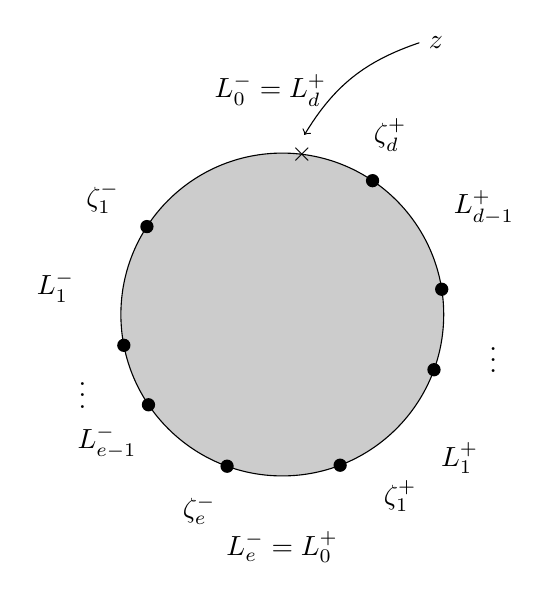
\begin{tikzpicture}[line cap=round,line join=round]
\draw[fill=gray!40] (0,0) circle (2.05);
\fill (147:2.05) circle (2.4pt);
\node at (147:2.72) {$\zeta^-_1$};
\node at (173:2.9) {$L^-_1$};
\fill (191:2.05) circle (2.4pt);
\node at (200:2.7) {$\vdots$};
\fill (214:2.05) circle (2.4pt);
\node at (216:2.75) {$L^-_{e-1}$};
\fill (250:2.05) circle (2.4pt);
\node at (247:2.7) {$\zeta^-_e$};
\node at (270:2.95) {$L^-_e=L^+_0$};
\fill (291:2.05) circle (2.4pt);
\node at (303:2.75) {$\zeta^+_1$};
\node at (321:2.9) {$L^+_1$};
\fill (340:2.05) circle (2.4pt);
\node at (350:2.72) {$\vdots$};
\fill (9:2.05) circle (2.4pt);
\node at (28:2.9) {$L^+_{d-1}$};
\fill (56:2.05) circle (2.4pt);
\node at (59:2.66) {$\zeta^+_d$};
\node at (83:2.05) {$\times$};
\node (zl) at (1.95,3.45) {$z$};
\draw[->] (zl.west) to[bend right=20] (0.28,2.28);
\node at (-0.15,2.85) {$L^-_0=L^+_d$};
\end{tikzpicture}
\caption{}\label{fig:even-incoming-disc}
\end{figure}
